\PostTableHeadingSpace
\section{Data and Knowledge Construction}

The reference implementation uses a bounded public-data slice to document how enterprise source material is turned into runtime knowledge. The section describes the company selection rule, source registration process, claim-promotion layer, and runtime claim set used for the paper baseline. The generated mobile briefing surface in \Cref{fig:ui-mobile-main} shows this data layer in product form: the selected state aligns the header price, news, stock, and filing-linked financial cards with the selected corporate group, and the selector callout shows the same surface switching across five groups.

\begin{figure}[H]
    \centering
    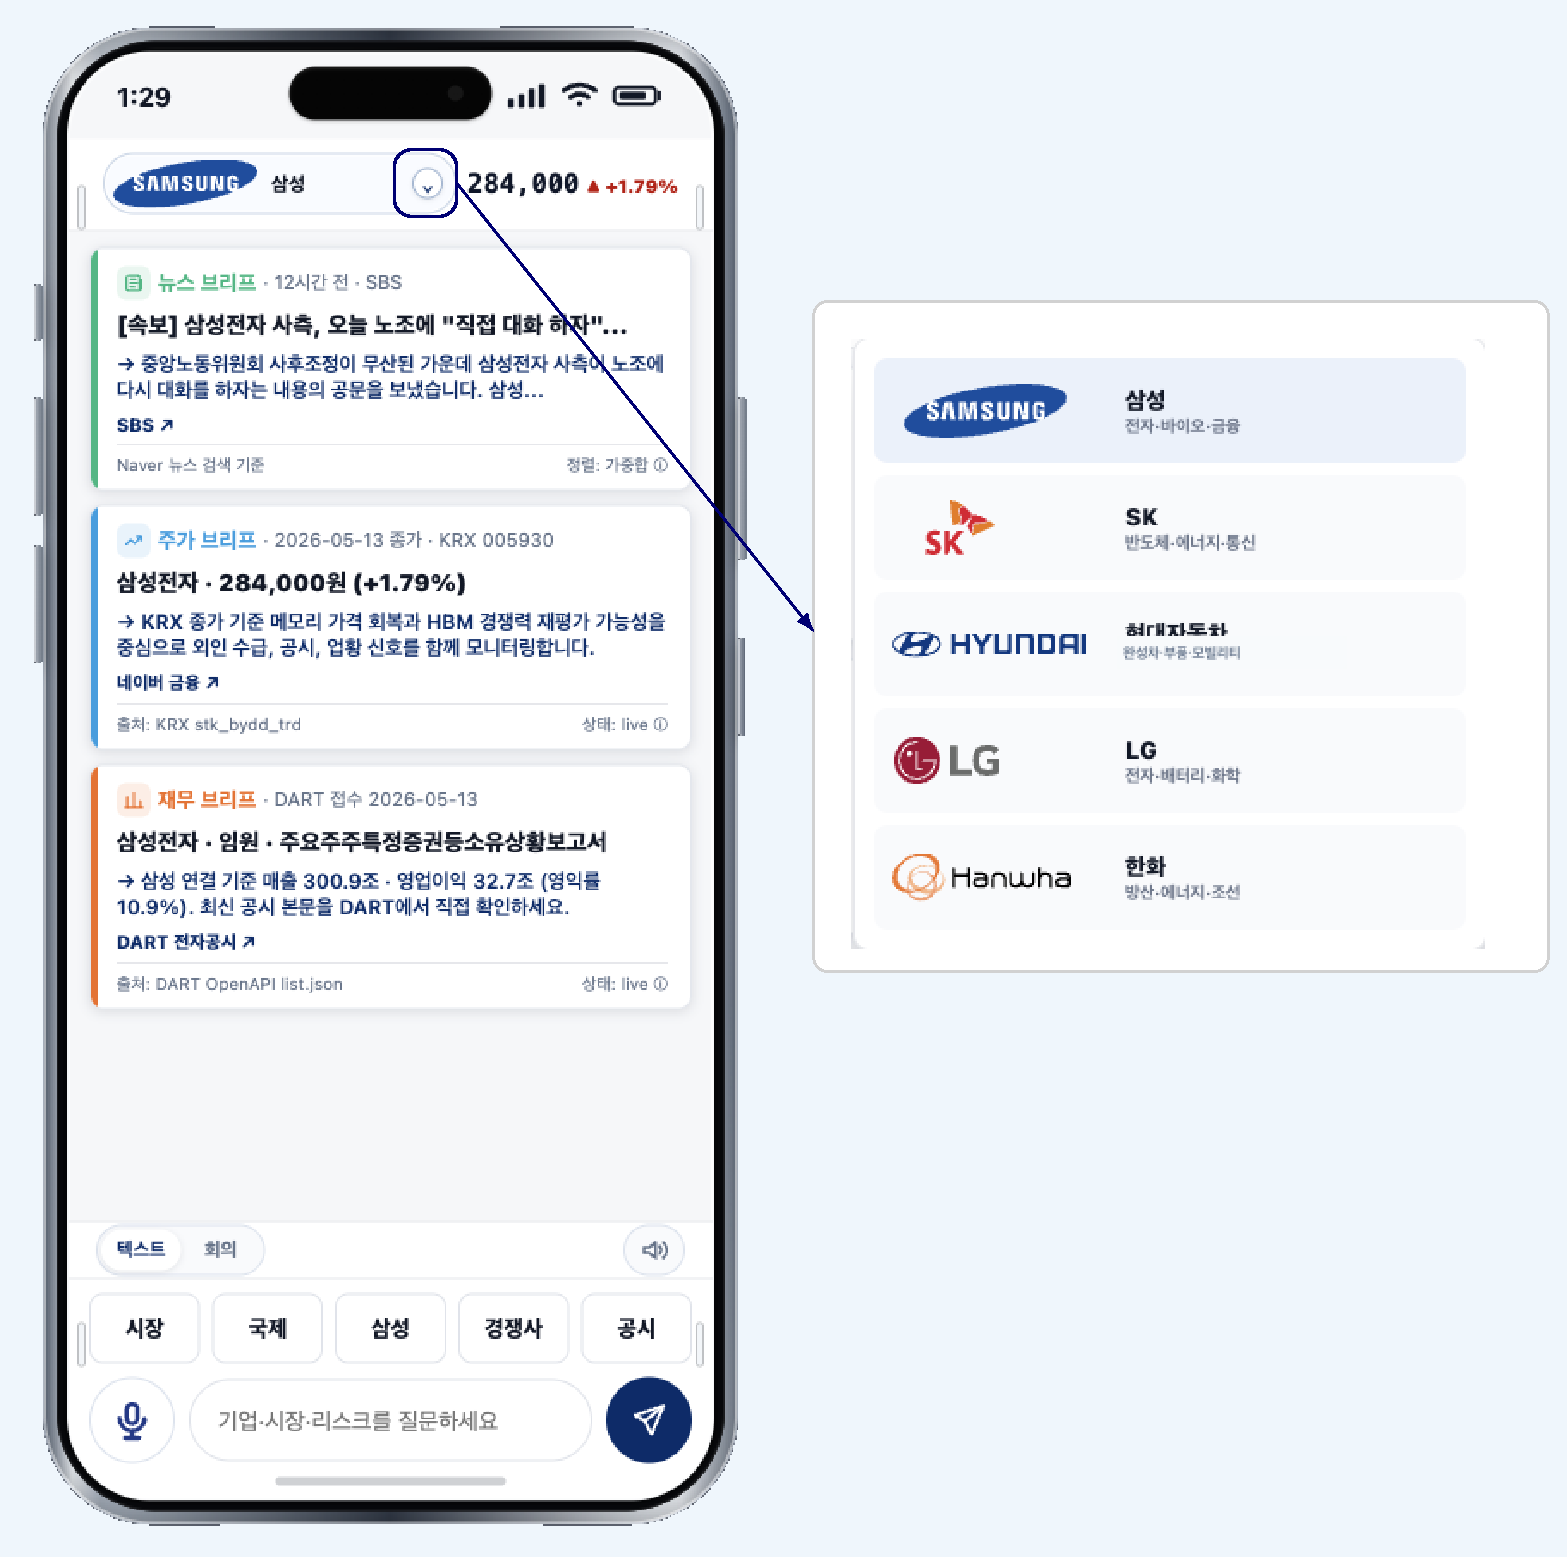
\includegraphics[width=0.95\linewidth]{figures/ui_mobile_main_ko_callout.pdf}
    \caption{Mobile main-screen briefing surface with selector callout. The selected Samsung state illustrates the shared interface, including news, stock, and filing-linked financial cards; the callout shows that the same surface switches among the five corporate groups.}
    \label{fig:ui-mobile-main}
\end{figure}

\subsection{Reference Company Slice}

The current slice covers five Korean corporate groups and five listed companies per corporate group. In this paper, a Korean corporate group refers to the corporate-group designation unit used by the Fair Trade Commission. The corporate-group boundary follows the 2026 ranking by fair-value assets in the official Fair Trade Commission designation results: Samsung, SK, Hyundai Motor, LG, and Hanwha form the top-five corporate-group set after Hanwha entered fifth place \citep{ftc2026businessgroups}. The ranking provides a reproducible sampling rule for the reference slice, independent of investment-quality assessment.

Within each corporate group, the five listed companies are selected by a fixed reference-slice policy. The policy prioritizes listed companies with stable KRX and OpenDART identifiers, corporate-group representativeness, sector diversity, comparability across corporate groups, public-source availability, claim-promotion feasibility, investor-facing relevance, and scope control. The five corporate groups test transfer across different source structures: affiliate-level IR pages, DART filings, holding-company materials, market-data interfaces, and news-search interfaces. The controlled 25-company slice supports routing and transferability tests while keeping source eligibility auditable. The selected companies and coverage focus used for the reference slice are defined in \Cref{tab:reference-slice-selection}.

\begin{table}[H]
    \centering
    \caption{Reference-slice company selection. Each corporate group contributes five listed companies selected for identifier readiness, representativeness, sector diversity, comparability, and source availability.}
    \label{tab:reference-slice-selection}
    \footnotesize
    \setlength{\tabcolsep}{4pt}
    \setlength{\extrarowheight}{1pt}
    \renewcommand{\arraystretch}{1.32}
    \begin{tabular}{@{}C{0.16\linewidth}
                    L{0.47\linewidth}
                    L{0.29\linewidth}@{}}
        \toprule
        \multicolumn{1}{C{0.16\linewidth}}{Corporate group} & \multicolumn{1}{C{0.47\linewidth}}{Selected listed companies} & \multicolumn{1}{C{0.29\linewidth}}{Coverage focus} \\
        \midrule
        Samsung & Samsung Electronics; Samsung SDI\newline Samsung C\&T; Samsung Biologics\newline Samsung Electro-Mechanics & Memory, battery, construction, bio, components \\
        \addlinespace[0.50em]
        SK & SK Hynix; SK Innovation; SK Inc.\newline SK Telecom; SK Square & Memory, energy, holding, telecom, ICT investment \\
        \addlinespace[0.50em]
        Hyundai Motor & Hyundai Motor; Kia; Hyundai Mobis\newline Hyundai Glovis; Hyundai Rotem & OEMs, parts, logistics, defense/rail \\
        \addlinespace[0.50em]
        LG & LG Electronics; LG Chem\newline LG Energy Solution; LG Innotek\newline LG Uplus & Electronics, materials, battery, components, telecom \\
        \addlinespace[0.50em]
        Hanwha & Hanwha Corp.; Hanwha Systems\newline Hanwha Aerospace; Hanwha Ocean\newline Hanwha Solutions & Holding, aerospace, energy, systems, shipbuilding \\
        \bottomrule
    \end{tabular}
\end{table}

Sources include issuer IR materials, earnings presentations, annual and periodic filings, governance documents, public filing URLs, market-data interfaces, and news-search interfaces. The raw public inputs used by the implementation fall into four practical classes: DART filings, issuer IR materials, KRX market rows, and news-search results. For Korean filing, market, and news data, the implementation uses OpenDART, Korea Exchange (KRX) OPEN API, and NAVER News Search as interface sources \citep{opendart2026api,krx2026openapi,naver2026newssearch}. DART and IR materials provide most promoted financial and corporate claims in the paper baseline, while KRX and news-search inputs provide runtime market and news signals that are linked, checked, and traced separately. A source is included in the runtime layer when it supports a claim class, fixed validation scenario, runtime feature, or onboarding requirement. Files discovered during official-site scans are recorded for provenance and are promoted into runtime use when they support a specific claim or validation need.

The broader source ledger is larger than the 25-company runtime slice. The ledger records company-level source metadata, public locators, local artifact pointers when available, provenance fields, selection reasons, and document-type classifications across the collected public materials. Source-inventory counts function as audit artifacts. Runtime answers depend on promoted claims, source manifests, and validation gates.

\subsection{Manifest and Claim Records}

Each source is first represented as a manifest entry with organizational scope, locator, source role, selection rule, and runtime policy, making source use auditable before synthesis occurs. Promoted claims are the runtime unit of factual knowledge: atomic source-backed statements with group and company scope, claim type, source evidence, runtime policy, and verification state. The \texttt{companyId} field supports affiliate-level routing so that a question about one affiliate is not answered with unrelated corporate-group evidence.

The source-to-claim promotion rule is illustrated by the worked example in \Cref{tab:source-to-claim-example} and generalized in the pipeline diagram in \Cref{fig:source-to-claim}. Samsung Electronics is used only as an illustrative example; the same rule is applied to all corporate groups in the reference slice.

\begin{table}[H]
    \centering
    \caption{Worked example of source-backed claim promotion.}
    \label{tab:source-to-claim-example}
    \footnotesize
    \setlength{\tabcolsep}{5pt}
    \renewcommand{\arraystretch}{1.22}
    \begin{tabular}{@{}C{0.18\linewidth}
                    L{0.76\linewidth}@{}}
        \toprule
        \multicolumn{1}{C{0.18\linewidth}}{Stage} & \multicolumn{1}{C{0.76\linewidth}}{Example} \\
        \midrule
        Registered source & Samsung Electronics 2024 consolidated financial statement from OpenDART, linked to the company and annual-report identifiers. \\
        \addlinespace[0.25em]
        Promoted claim & The extracted DART row is promoted into a source-backed claim: 2024 consolidated revenue KRW 300.9 trillion and operating income KRW 32.7 trillion. \\
        \addlinespace[0.25em]
        Runtime use & The claim can support margin, trend, or portfolio questions. The reader sees the interpreted answer and source link, while claim IDs and trace metadata remain in the audit layer. \\
        \bottomrule
    \end{tabular}
\end{table}

\begin{figure}[!t]
    \centering
    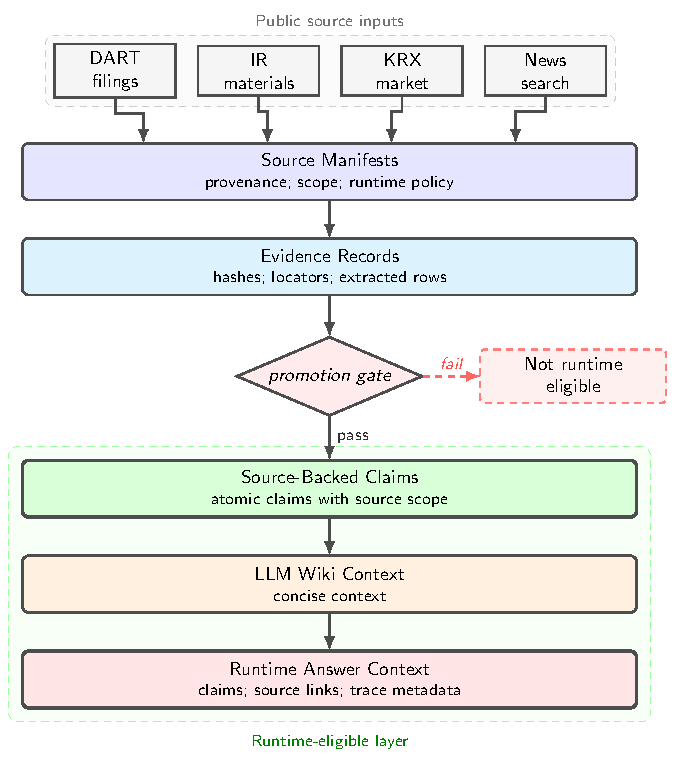
\includegraphics[width=0.95\linewidth,height=0.62\textheight,keepaspectratio]{figures/source_to_claim_pipeline.pdf}
    \caption{Source-to-claim pipeline. DART filings, issuer IR materials, KRX market rows, and news-search results are registered as source manifests before they are promoted as source-backed claims or attached as traceable runtime signals.}
    \label{fig:source-to-claim}
\end{figure}

\subsection{Runtime Claim Layer}

The source-backed runtime layer used in the case study is summarized in \Cref{tab:data-artifacts}. Runtime claims are the promoted, source-backed statements that the answer composer is allowed to use at runtime. They are distinct from raw document counts, extracted sentence counts, and company-importance measures. The claim counts are intentionally smaller than the number of collected files because they count only statements that passed source-linking and runtime-promotion gates. Differences across corporate groups reflect how many source-backed statements were promoted for the current fixed validation scenarios and answer templates.

The counts exclude downloaded files, extracted text, wiki pages, and unpromoted claim candidates. Most promoted claims in this baseline come from OpenDART records and selected official IR materials; market and news inputs are handled as runtime signals.

The five-corporate-group manifests currently contain 113 source-backed runtime claims. A compact 25-claim review-selected reference layer, five priority claims per corporate group, is used for paper reporting and product inspection. The 25-claim layer keeps reported coverage tied to selected evidence while still making transfer progress measurable: the ledger documents the wider source inventory, while the runtime layer uses only promoted, source-linked claims.

\begin{table}[H]
    \centering
    \caption{Source-backed runtime claim layer in the reference implementation.}
    \label{tab:data-artifacts}
    \footnotesize
    \setlength{\tabcolsep}{3pt}
    \renewcommand{\arraystretch}{1.25}
    \begin{tabular}{@{}C{0.15\linewidth}
                    C{0.13\linewidth}
                    L{0.31\linewidth}
                    L{0.29\linewidth}@{}}
        \toprule
        \multicolumn{1}{C{0.15\linewidth}}{Corporate group} & \multicolumn{1}{C{0.13\linewidth}}{Runtime claims} & \multicolumn{1}{C{0.31\linewidth}}{Claim coverage} & \multicolumn{1}{C{0.29\linewidth}}{Validation role} \\
        \midrule
        Samsung & 36 & Memory/electronics, battery, construction, bio, components & Tests routing across the broadest affiliate mix in the slice \\
        \addlinespace[0.35em]
        SK & 27 & Memory, energy, holding-company, telecom, ICT investment & Tests semiconductor and portfolio-allocation questions \\
        \addlinespace[0.35em]
        Hyundai Motor & 15 & OEMs, parts, logistics, defense/rail & Tests mobility-centered affiliate routing and source separation \\
        \addlinespace[0.35em]
        LG & 15 & Electronics, materials, battery, components, telecom & Tests electronics-battery-materials coverage with telecom cash-flow context \\
        \addlinespace[0.35em]
        Hanwha & 20 & Holding, aerospace, energy, systems, shipbuilding & Tests defense, energy, and shipbuilding claims under one corporate-group boundary \\
        \bottomrule
    \end{tabular}
\end{table}
\FloatBarrier
